\documentclass[11pt,letterpaper]{article}
\usepackage[margin=1in]{geometry}
\usepackage{mathptmx}
\usepackage{graphicx}
\usepackage{booktabs}
\usepackage{tikz}
\usetikzlibrary{arrows.meta,positioning}
\usepackage[hidelinks]{hyperref}
\hypersetup{pdftitle={Preserving Visual Evidence in Compressed Multimodal Reasoning}}
\setlength{\parindent}{0pt}
\setlength{\parskip}{3pt}
\makeatletter
\renewcommand\section{\@startsection{section}{1}{\z@}{-2ex plus -.5ex minus -.2ex}{1ex plus .2ex}{\normalfont\large\bfseries}}
\makeatother
\setlength{\textfloatsep}{10pt}
\setlength{\intextsep}{9pt}
\newcommand{\ind}{\mathbf{1}}
\newcommand{\arxiv}[1]{\href{https://arxiv.org/abs/#1}{arXiv:#1}}
\begin{document}
\begin{center}
{\Large\bfseries Preserving Visual Evidence in Compressed Multimodal Reasoning\par}
\vspace{5pt}
{\normalsize Research Proposal}
\end{center}
\vspace{-8pt}
\section*{Abstract}
Concise multimodal reasoning can omit a visual premise while stating only correct steps. We will test an image-aware sufficiency reward that detects this missing support. Four reward arms will share compressed cold-start data, initialization, budget conditioning, and measured policy-training compute: sufficiency, style, stated-step correctness, and zero auxiliary reward. Using Qwen2.5-VL-7B-Instruct, we will study 3,000 geometry and bar-chart problems with independent human evaluation and checked image interventions. Near 128 achieved reasoning tokens, the primary target is a 3-point accuracy gain and a 5-point human-sufficiency gain over style supervision. A judge gate and throughput pilot precede training within a 400 accelerator-hour cap.

\section{Introduction}
Compression saves generated text, but a useful explanation must retain the facts supporting its answer. In visual mathematics, those facts include readings and relations available only in a diagram. A trace can contain valid arithmetic yet omit the visual premises that make the calculation applicable. Chain-of-thought prompting and reinforcement learning motivate studying the intermediate reasoning as well as final correctness \cite{wei,deepseek}.

SketchThinker-R1 \cite{sketch} trains concise multimodal reasoning with a text-only style judge. Its answering policy sees images and questions; SketchJudge sees neither. Appendix~H evaluates key-step preservation in cold-start sketches: Table~14 classifies 19,182 as preserving key steps and 818 as missing them. The remaining gap concerns omission-sensitive supervision and independent sufficiency evaluation of learned-policy outputs, including wrong answers.

The paper's 7B results show large token savings, while its 3B MathVision comparison falls from 26.9\% to 25.3\% accuracy (Table~2). This variation motivates measuring accuracy and explanatory support separately. We ask: (RQ1) which necessary visual premises disappear relative to nonvisual units, allowing alternative derivations? (RQ2) does omission-sensitive supervision improve accuracy and sufficiency beyond style and stated-step correctness at matched lengths and compute? (RQ3) do gains persist on image interventions and under separate image-access and omission-training ablations?

\section{Related Work}
\textbf{Compression and allocation.} Sketch-of-Thought compresses reasoning through constrained paradigms \cite{sot}; s1 controls test-time computation through budget forcing \cite{sone}. SketchThinker-R1 combines rewriting, cold start, and reinforcement learning, with default reward weights of 0.5 accuracy, 0.4 format, and 0.1 style \cite{sketch}. Its stage, judge, schedule, and long-trace controls establish useful comparisons; a shared-initialization reward contrast tests the incremental value of the auxiliary signal.

\textbf{Correct steps and complete support.} Process supervision checks intermediate steps \cite{lightman}; VisualPRM extends process reward modeling to multimodal reasoning \cite{visualprm}. We distinguish correctness of stated steps from whether the trace supplies all premises needed for its returned answer. MathVerse varies diagram/text information \cite{mathverse}; MathVista and MATH-Vision provide visual-mathematics transfer settings \cite{mathvista,mathvision}. Qwen2.5-VL supplies the policy and judge backbones \cite{qwen}, with GRPO for policy optimization \cite{grpo}. Explanatory sufficiency is observable support; causal faithfulness requires a different test \cite{turpin}.

\newpage
\section{Proposed Methodology}
\textbf{Explicit sufficiency.} Given image $I$ and question $q$, policy $\pi_\theta$ returns trace $z$ and answer $a$. All explanation preceding the normalized answer counts toward reasoning length $L(z)$. Reviewers annotate a set $\mathcal{G}(I,q)$ of admissible derivation graphs, accepting valid alternative proofs. Nodes represent visual premises, question facts, and deductions; visual nodes carry region references or measurable relations. A unit is necessary relative to a derivation when removing it breaks support for the answer.

For graph $G$, let $P_{V,G}(z)$ and $P_{N,G}(z)$ be fractions of required visual premises and nonvisual units explicitly stated and correct. Let $D_G(z)$ indicate valid deductions supporting the returned answer from these premises, question facts, and declared elementary rules. Define
\begin{equation}
S(z;I,q,\mathcal{G})=\max_{G\in\mathcal{G}(I,q)}
\ind[P_{V,G}(z)=1]\,\ind[P_{N,G}(z)=1]D_G(z).
\label{eq:suff}
\end{equation}
The image checks stated facts without filling omissions. Thus a triangle calculation silently importing image-only angle readings is incomplete. Redundant deletions pass when a complete valid derivation remains. Empty unit categories have coverage one; category summaries exclude them and report their counts. Newly identified valid proofs enter blinded adjudication under the same rubric.

\begin{figure}[ht]
\centering
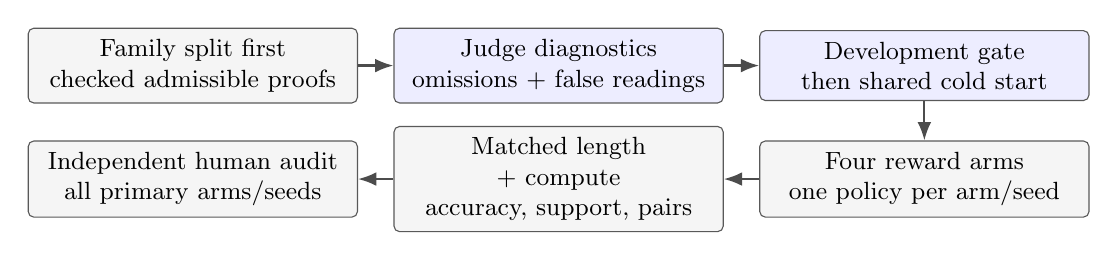
\begin{tikzpicture}[font=\small,>=Latex,
 box/.style={draw=black!65,rounded corners=2pt,align=center,text width=3.9cm,minimum height=.85cm,inner sep=4pt},
 flow/.style={->,thick,draw=black!70}]
\node[box,fill=black!4] (data) {Family split first\\checked admissible proofs};
\node[box,fill=blue!7,right=.45cm of data] (judge) {Judge diagnostics\\omissions + false readings};
\node[box,fill=blue!7,right=.45cm of judge] (gate) {Development gate\\then shared cold start};
\node[box,fill=black!4,below=.5cm of gate] (rl) {Four reward arms\\one policy per arm/seed};
\node[box,fill=black!4,left=.45cm of rl] (eval) {Matched length + compute\\accuracy, support, pairs};
\node[box,fill=black!4,left=.45cm of eval] (human) {Independent human audit\\all primary arms/seeds};
\draw[flow] (data)--(judge);\draw[flow] (judge)--(gate);\draw[flow] (gate)--(rl);
\draw[flow] (rl)--(eval);\draw[flow] (eval)--(human);
\end{tikzpicture}
\caption{Proposed study. Training annotations supervise judges; development data calibrate and select settings; held-out human labels evaluate generated traces.}
\label{fig:pipeline}
\end{figure}

\textbf{Judge and comparator.} Initialize judges from Qwen2.5-VL-3B. Sufficiency and stated-step correctness judges receive identical $I,q,z,a$ inputs, without the gold answer. The correctness judge checks stated propositions and deductions; sufficiency additionally requires complete support. The style judge receives trace text alone. Training contrasts complete sketches, correct-answer premise deletions, false readings, invalid deductions, redundant deletions, and alternative proofs, matching length and format. Structured grounding/deduction labels and binary judgments use supervised cross-entropy. Development calibration selects a binary threshold requiring false acceptance $\leq10\%$ and sufficient-trace recall $\geq70\%$. Failure returns the study to labeling and diagnostics before RL.

\textbf{Common policy objective.} Four arms share Qwen2.5-VL-7B-Instruct compressed cold-start weights and data. With $A_\phi$ denoting each binary auxiliary judgment, use
\begin{equation}
R=0.5\ind[a=a^*]+0.4F(z,a)+0.1A_\phi-\lambda\max(0,L(z)/B-1).
\label{eq:reward}
\end{equation}
The zero-auxiliary arm sets $A_\phi=0$ without renormalization. GRPO uses shared rollout settings and a KL anchor to the cold-start policy. Common budget conditioning targets $B\in\{64,128,256\}$ within each trained policy. The pilot fixes length-penalty search and throughput settings before the primary runs; deployment uses the policy alone.

\newpage
\section{Experimental Plan}
\textbf{Data and split.} Render 3,000 verifiable geometry and bar-chart problems, assigning 1,600 to training, 400 to development, and 1,000 to test. Split by template family before generating traces or image variants. Generators supply checked reference facts and derivations. Two annotators independently audit 300 test problems, adjudicate alternative proofs, and blindly score outputs from every primary arm and seed, including wrong answers. Report agreement before adjudication. Development annotations calibrate the judges; test annotations remain outside fitting and selection.

\textbf{Controlled reward comparison.} Sufficiency, style, stated-step correctness, and zero auxiliary reward share source problems, compressed SFT data, cold-start initialization, accuracy/format coefficients, and tuning allowance. Match measured policy-training accelerator-hours, including rollouts and judge scoring. A fixed-rollout sensitivity check complements the compute-matched comparison. Match achieved mean reasoning lengths within 5\% using development-only operating-point selection. Freeze prompts, image resolution, decoding, answer parser, and settings before test access; report unmatched points separately. Include long-reasoning and direct-answer references.

\textbf{Interventions and ablations.} Independently construct 200 answer-changing and 100 nuisance-edit pairs from held-out originals. Validate both images, their answers, and preservation of unrelated facts. Regenerate traces for both members; measure both-correct answers and valid support in each image. Shared relational wording passes when valid for both. Nuisance edits test invariance. Separately remove judge image access and omission-negative training; compare these and the stated-step control against the useful-effect thresholds. These contrasts test the proposed mechanisms while independent human labels check reward exploitation.

\begin{table}[ht]
\centering\small
\caption{Planned evaluation; all counts and operating points are design choices.}
\begin{tabular}{@{}p{.25\linewidth}p{.34\linewidth}p{.34\linewidth}@{}}
\toprule
\raggedright Dataset / role & \raggedright Measures & \raggedright Comparison \tabularnewline
\midrule
\raggedright Rendered family-held-out test; 1,000 problems & \raggedright Accuracy, achieved length, visual/nonvisual retention, grounding errors & \raggedright Four shared-cold-start arms; three seeds each \tabularnewline
\raggedright Human audit; 300 test problems & \raggedright Explicit sufficiency, valid deductions, alternative proofs & \raggedright Blinded scoring of every primary arm/seed, including wrong answers \tabularnewline
\raggedright 200 answer-changing and 100 nuisance pairs & \raggedright Both-correct rate, valid support, nuisance invariance & \raggedright Same arms; separate image-access and omission-training ablations \tabularnewline
\raggedright Public tests, reserved for transfer & \raggedright Official accuracy, length, end-to-end latency & \raggedright Long reasoning and direct answers; separate checkpoint exposure record \tabularnewline
\bottomrule
\end{tabular}
\label{tab:experiments}
\end{table}

\textbf{Omission and retention.} For RQ1, condition omission analysis on retained admissible derivations. Let $U_C$ be necessary units explicit and correct in the original trace, for category $C\in\{V,N\}$. If $M_u(z_c)$ indicates a semantic mention in compressed trace $z_c$, define
\[
d_C^{\rm omit}=1-\frac{1}{|U_C|}\sum_{u\in U_C}M_u(z_c),\qquad |U_C|>0.
\]
Macro-average over nonempty problems and report empty-category counts. Score false readings, invalid deductions, and valid proof changes separately; an omitted unit differs from a stated but incorrect one. RQ2 evaluates final accuracy and human sufficiency separately, alongside necessary visual/nonvisual premise retention. Judge false acceptance on unsupported traces remains a diagnostic outcome.

\textbf{Transfer.} Reserve public tests for transfer and record checkpoint exposure. Use full MathVision; MathVista requires an item-level overlap audit because SketchRL-1K draws from it \cite{sketch,mathvista}. MathVerse checks diagram dependence within the cap.

\newpage
\textbf{Success and uncertainty.} Near 128 achieved reasoning tokens, the primary sufficiency-versus-style contrast must gain at least 3 percentage points in accuracy and 5 points in human-rated sufficiency. Both paired 95\% confidence intervals must lie above zero. Prespecify this contrast and adjust secondary comparisons for multiplicity. Report each of three training seeds, its effect, and the seed-effect range. Paired intervals cluster by original problem family, keeping image variants together; these intervals describe item-sampling uncertainty separately from training variation.

Pilot paired/clustered precision before freezing the protocol. The test size and compute ceiling do not guarantee resolution of the useful-effect thresholds. An interval spanning useful gains and losses leaves the comparison unresolved; an interval ruling out a useful gain bounds its practical value. Retention gains without accuracy gains support an explanation-quality contribution. Prespecified derivation-depth and visual-dependency groups expose subgroup losses that aggregate means conceal.

\textbf{Latency and cost.} Time from prepared-input receipt through final answer, including vision encoding, image/text prefill, reasoning, and answer decoding. Randomize warmed-up timing order on fixed hardware/software, resolution, and batching. Record preparation, shared SFT, judge fitting/scoring, rollout generation, and policy updates in a unified ledger. Report accelerator-hours and API spending separately, along with processed image/text tokens. The primary compute match includes rollout and judge inference; equal update counts alone do not establish equality.

\section{Expected Results \& Timeline}
We predict that omission-sensitive supervision will retain explicit visual support and improve accuracy under compression. The stated-step baseline determines whether completeness adds value beyond checking what the trace already says. The image-access and omission-negative ablations test the intended supervision mechanisms. Independent trace ratings, alternative proofs, and image pairs define where any benefit holds; the study also reports calibrated judges and useful null results.

Use LoRA on two 80GB accelerators with a total cap of 400 accelerator-hours: 12 principal runs (four arms $\times$ three seeds) at 25 hours each consume 300, leaving 100 for judges, shared preparation, selection, diagnostics, evaluation, and ablations. Hours sum occupancy across all accelerators; 25 accelerator-hours on two devices is 12.5 wall hours. Begin with judge discrimination and frozen-policy diagnostics. Pilot throughput before RL; reduce data/steps equally if required, preserving three seeds and the primary contrast. One budget-conditioned policy covers all operating points in each run.

\begin{table}[ht]
\centering\small
\caption{Six-month milestones within the shared resource ceiling.}
\label{tab:timeline}
\begin{tabular}{@{}p{.08\linewidth}p{.84\linewidth}@{}}
\toprule
Month & Activities and decision points \\
\midrule
1 & Judge/frozen-policy diagnostics; throughput and precision pilots; freeze split and rubric. \\
2 & Render problems; annotate derivations; independently validate image pairs. \\
3 & Calibrate judges; pass false-acceptance and recall gate before policy training. \\
4 & Train four reward arms with three seeds and common budget conditioning. \\
5 & Freeze operating points; evaluate held-out families, transfer, and separate ablations. \\
6 & Complete blinded human audit, uncertainty analysis, cost ledger, and release. \\
\bottomrule
\end{tabular}
\end{table}

Outputs will include permitted data and image edits, generators, annotation rubrics, judge calibration, policy configurations, and accuracy--length curves. The final report will identify the conditions where sufficiency supervision improves compressed reasoning and those where it offers no advantage.

\clearpage
\begin{thebibliography}{13}
\small
\bibitem{wei} Jason Wei, Xuezhi Wang, Dale Schuurmans, Maarten Bosma, Brian Ichter, Fei Xia, Ed Chi, Quoc Le, and Denny Zhou. 2022. Chain-of-Thought Prompting Elicits Reasoning in Large Language Models. \arxiv{2201.11903}. Conference version: \emph{NeurIPS}, 2022.
\bibitem{deepseek} DeepSeek-AI, Daya Guo, Dejian Yang, Haowei Zhang, et al. 2025. DeepSeek-R1: Incentivizing Reasoning Capability in LLMs via Reinforcement Learning. \arxiv{2501.12948}. Published version: \emph{DeepSeek-R1 incentivizes reasoning in LLMs through reinforcement learning}, \emph{Nature} 645, 633--638 (2025), \href{https://doi.org/10.1038/s41586-025-09422-z}{doi:10.1038/s41586-025-09422-z}.
\bibitem{sketch} Ruiyang Zhang, Dongzhan Zhou, and Zhedong Zheng. 2026. SketchThinker-R1: Towards Efficient Sketch-Style Reasoning in Large Multimodal Models. In \emph{International Conference on Learning Representations (ICLR)}, 2026. \href{https://openreview.net/forum?id=ZSMDuKtYbt}{OpenReview}; also \arxiv{2601.02825}.
\bibitem{sot} Simon A. Aytes, Jinheon Baek, and Sung Ju Hwang. 2025. Sketch-of-Thought: Efficient LLM Reasoning with Adaptive Cognitive-Inspired Sketching. \arxiv{2503.05179}.
\bibitem{sone} Niklas Muennighoff, Zitong Yang, Weijia Shi, Xiang Lisa Li, Li Fei-Fei, Hannaneh Hajishirzi, Luke Zettlemoyer, Percy Liang, Emmanuel Cand\`es, and Tatsunori Hashimoto. 2025. s1: Simple test-time scaling. \arxiv{2501.19393}.
\bibitem{lightman} Hunter Lightman, Vineet Kosaraju, Yura Burda, Harri Edwards, Bowen Baker, Teddy Lee, Jan Leike, John Schulman, Ilya Sutskever, and Karl Cobbe. 2023. Let's Verify Step by Step. \arxiv{2305.20050}. Conference version: \emph{ICLR}, 2024.
\bibitem{turpin} Miles Turpin, Julian Michael, Ethan Perez, and Samuel R. Bowman. 2023. Language Models Don't Always Say What They Think: Unfaithful Explanations in Chain-of-Thought Prompting. \arxiv{2305.04388}. Conference version: \emph{NeurIPS}, 2023.
\bibitem{mathverse} Renrui Zhang, Dongzhi Jiang, Yichi Zhang, Haokun Lin, Ziyu Guo, Pengshuo Qiu, Aojun Zhou, Pan Lu, Kai-Wei Chang, Peng Gao, and Hongsheng Li. 2024. MathVerse: Does Your Multi-modal LLM Truly See the Diagrams in Visual Math Problems? \arxiv{2403.14624}. Conference version: \emph{ECCV}, 2024.
\bibitem{mathvista} Pan Lu, Hritik Bansal, Tony Xia, Jiacheng Liu, Chunyuan Li, Hannaneh Hajishirzi, Hao Cheng, Kai-Wei Chang, Michel Galley, and Jianfeng Gao. 2023. MathVista: Evaluating Mathematical Reasoning of Foundation Models in Visual Contexts. \arxiv{2310.02255}. Conference version: \emph{ICLR}, 2024.
\bibitem{mathvision} Ke Wang, Junting Pan, Weikang Shi, Zimu Lu, Mingjie Zhan, and Hongsheng Li. 2024. Measuring Multimodal Mathematical Reasoning with MATH-Vision Dataset. \arxiv{2402.14804}. Conference version: \emph{NeurIPS, Datasets and Benchmarks Track}, 2024.
{\raggedright\bibitem{qwen} Shuai Bai, Keqin Chen, Xuejing Liu, Jialin Wang, et al. 2025. Qwen2.5-VL Technical Report. \arxiv{2502.13923}.\par}
\bibitem{grpo} Zhihong Shao, Peiyi Wang, Qihao Zhu, Runxin Xu, Junxiao Song, Xiao Bi, Haowei Zhang, Mingchuan Zhang, Y.K. Li, Y. Wu, and Daya Guo. 2024. DeepSeekMath: Pushing the Limits of Mathematical Reasoning in Open Language Models. \arxiv{2402.03300}.
\bibitem{visualprm} Weiyun Wang, Zhangwei Gao, Lianjie Chen, Zhe Chen, Jinguo Zhu, Xiangyu Zhao, Yangzhou Liu, Yue Cao, Shenglong Ye, Xizhou Zhu, Lewei Lu, Haodong Duan, Yu Qiao, Jifeng Dai, and Wenhai Wang. 2026. VisualPRM400K: An Effective Dataset for Training Multimodal Process Reward Models. \emph{ICLR}. Preprint: \emph{VisualPRM: An Effective Process Reward Model for Multimodal Reasoning} (2025), \arxiv{2503.10291}.
\end{thebibliography}
\end{document}
